\documentclass[10pt]{beamer}

% Beamer style
%\usetheme[secheader]{Madrid}
\usetheme{CambridgeUS}
\usecolortheme[rgb={0.65,0.15,0.25}]{structure}
%\usefonttheme[onlymath]{serif}
\beamertemplatenavigationsymbolsempty
%\AtBeginSubsection

% Packages
%\usepackage[french]{babel}
\usepackage[latin1]{inputenc}
\usepackage{color}
\usepackage{dsfont, stmaryrd}
\usepackage{amsmath, amsfonts, amssymb}
\usepackage{stmaryrd}
\usepackage{epsfig}
\usepackage{/home/robin/LATEX/Biblio/astats}
%\usepackage[all]{xy}
\usepackage{graphicx}

% Commands
\definecolor{darkred}{rgb}{0.65,0.15,0.25}
\definecolor{darkgreen}{rgb}{0,0.4,0}
\newcommand{\emphase}[1]{\textcolor{darkred}{#1}}
%\newcommand{\emphase}[1]{\textcolor{black}{#1}}
\newcommand{\paragraph}[1]{\textcolor{darkred}{#1}}
\newcommand{\refer}[1]{\textcolor{blue}{[\cite{#1}]}}
\newcommand{\Refer}[1]{\textcolor{blue}{[#1]}}
% \newcommand{\newblock}{}

% Symbols
\newcommand{\Bcal}{\mathcal{B}}
\newcommand{\dd}{\text{d}}
\newcommand{\Esp}{\mathbb{E}}
\newcommand{\Kbf}{{\bf K}}
\newcommand{\Gcal}{\mathcal{G}}
\newcommand{\Gam}{\mathcal{G}\text{am}}
\newcommand{\Ibb}{\mathbb{I}}
\newcommand{\Var}{\mathbb{V}}
\newcommand{\Fcal}{\mathcal{F}}
\newcommand{\Hcal}{\mathcal{H}}
\newcommand{\Lcal}{\mathcal{L}}
\newcommand{\Mcal}{\mathcal{M}}
\newcommand{\Ncal}{\mathcal{N}}
\newcommand{\Nbf}{{\bf N}}
\newcommand{\Nm}{N(\mbf)}
\newcommand{\Ocal}{\mathcal{O}}
\newcommand{\Obf}{{\bf 0}}
\newcommand{\Omegas}{\underset{s}{\Omega}}
\newcommand{\Ybf}{{\bf Y}}
\newcommand{\Pcal}{\mathcal{P}}
\newcommand{\Qcal}{\mathcal{Q}}
\newcommand{\Rbb}{\mathbb{R}}
\newcommand{\Rcal}{\mathcal{R}}
\newcommand{\sbf}{{\bf s}}
\newcommand{\Sbf}{{\bf S}}
\newcommand{\Scal}{\mathcal{S}}
\newcommand{\Ucal}{\mathcal{U}}
\newcommand{\Vcal}{\mathcal{V}}
\newcommand{\cst}{\text{cst}}
\newcommand{\ra}{\emphase{$\rightarrow$~}}

\newcommand{\fignet}{/home/robin/RECHERCHE/RESEAUX/EXPOSES/FIGURES/}

%====================================================================
\title[Change-point problems in genomics]{Change-point problems in genomics}

\author[S. Robin]{S. Robin \\  }

\institute[AgroParisTech / INRA]{
  {\normalsize \begin{tabular}{rl}
    joint works with & E. Lebarbier, G. Rigaill \\
    & A. Cleynen \\
    & M. Delattre, C. L�vy-Leduc, T. Mary-Huard
    \end{tabular}} \\

  \bigskip
 \begin{tabular}{ccccc}
    
\includegraphics[width=.2\textwidth]{../FIGURES/LogoINRA-Couleur} & 
    \hspace{.02\textwidth} &
    
\includegraphics[width=.3\textwidth]{../FIGURES/logagroptechsolo} & 
    \hspace{.02\textwidth} &
    
\includegraphics[width=.2\textwidth]{../FIGURES/logo-ssb} \\ 
  \end{tabular} \\
  \bigskip 
  }

  \date[Ispahan, 2016]{Ispahan, 2016}

%====================================================================

%====================================================================
%====================================================================
\begin{document}
%====================================================================
%====================================================================

%====================================================================
\frame{\titlepage
  }

% %====================================================================
% \frame{\frametitle{Outline} 
%   \tableofcontents
%   }

%====================================================================
%====================================================================
\section[Change point problems in genomics]{Change point problems in genomics: Main issues}
%====================================================================
\frame{\frametitle{Change point problems in genomics: Main issues} 

  \paragraph{Genomic data:} often collected 'along the genome', similarly to time series
  
  \bigskip \bigskip
  \paragraph{Genomic experiments:} often aim at finding regions in which some specific event occurs:
  \begin{itemize}
   \item copy number variations (gain or loss of genomic regions)
   \item gene detection (detection of transcribed region)
   \item protein-DNA interactions (e.g. detection of protein biding sites)
   \item ...
  \end{itemize}

  \bigskip \medskip
  \paragraph{Genomic technologies} now provide information at the nucleotide resolution
  }

%====================================================================
\frame{\frametitle{Different experiments and technologies} 

  \begin{tabular}{l}
    \vspace{-.05\textheight}
    \paragraph{Comparative genomic hypridization:} microarrays / copy number variation \\ ~
    \begin{tabular}{c}
	 \begin{overprint}
	   \onslide<1>
	   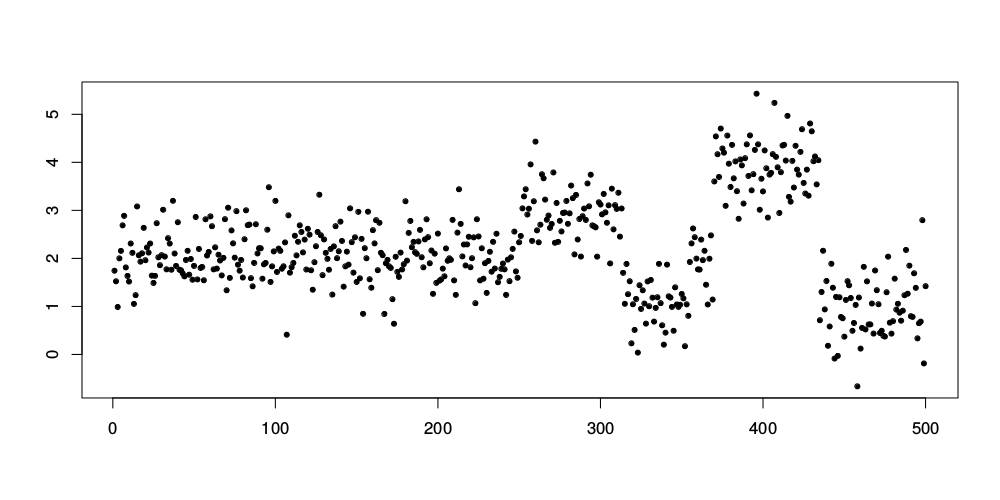
\includegraphics[height=.45\textheight, width=.9\textwidth]{../FIGURES/FigSeg-Cambridge-CGH.pdf}
	   \onslide<2>
	   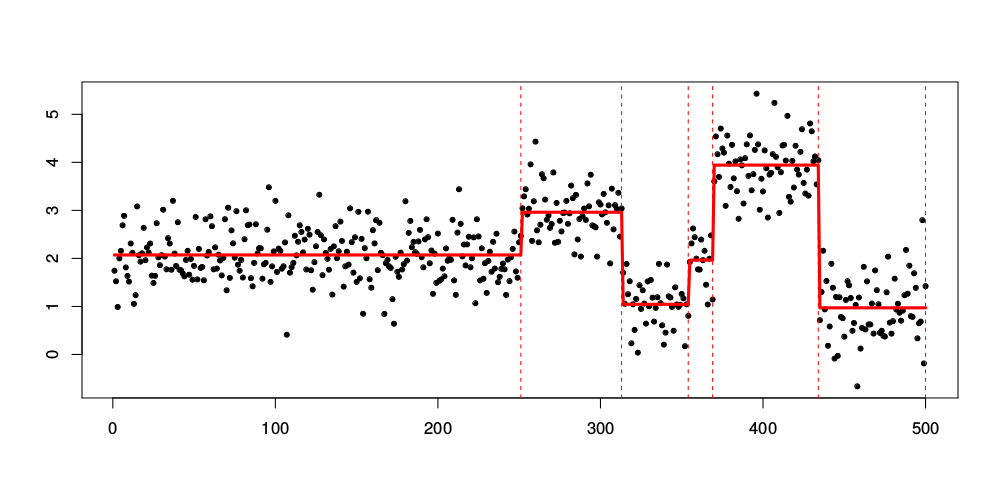
\includegraphics[height=.45\textheight, width=.9\textwidth]{../FIGURES/FigSeg-Cambridge-CGH-seg.pdf}
	 \end{overprint}
    \end{tabular}
    \\
    \vspace{-.05\textheight}
    \paragraph{RNA-sequencing:} massive sequencing / gene expression \\ ~
    \begin{tabular}{c}
	 \begin{overprint}
	   \onslide<1>
	   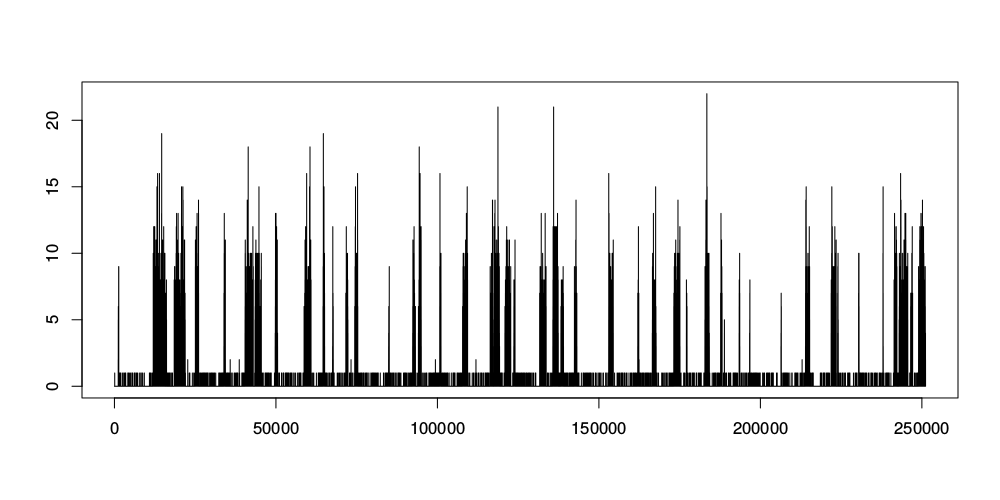
\includegraphics[height=.45\textheight, width=.9\textwidth]{../FIGURES/FigSeg-Cambridge-RNAseq.pdf}
	   \onslide<2>
	   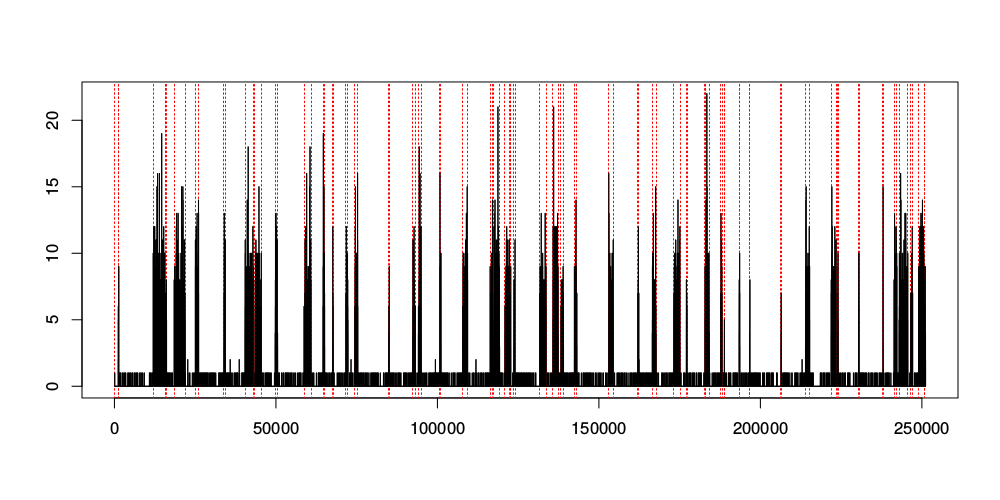
\includegraphics[height=.45\textheight, width=.9\textwidth]{../FIGURES/FigSeg-Cambridge-RNAseq-seg.pdf}
    \end{overprint}
    \end{tabular}
  \end{tabular}
  }

%====================================================================
\frame{\frametitle{Two scales} 

  \paragraph{Global scale: $n \approx 10^6 - 10^8$} (whole genome) \\
  Aim = find the 'best' segmentation, not much more.
  \begin{itemize}
   \item Need for efficient algorithms (not quadratic!): \refer{KFE12}, \refer{CKL14} 
   \item Need for a dedicated criterion to choose $K$: see \refer{ClL14}, \refer{ZhS07} 
  \end{itemize}

  \bigskip \bigskip 
  \paragraph{Local scale: $n \approx 10^3$} (genomic region) \\
  Aim = answer to more precise questions
  \begin{itemize}
   \item Reliability of the 'best' segmentation
   \item Confidence intervals for the change points
   \item Change point comparison
  \end{itemize}
  }


%====================================================================
%====================================================================
\section{Global scale}
%====================================================================
\frame{\frametitle{Global scale: comparative study for SNP arrays}

  \paragraph{Benchmark of manually annotated profiles:} ROC curves \refer{Hoc12}
  $$
  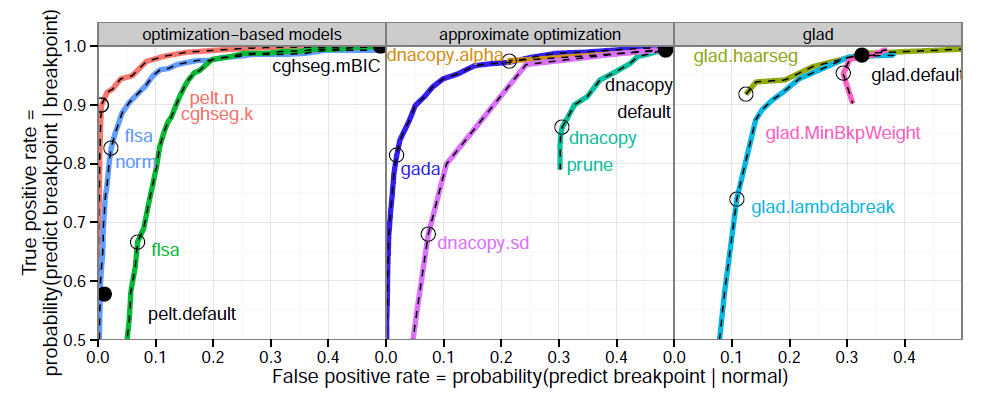
\includegraphics[width=\textwidth]{../FIGURES/Hoc12-Fig3-3}     
  $$
 }

%====================================================================
\frame{\frametitle{Application: Copy number variations \& breast cancer}

  $$
  \begin{tabular}{cc}
    Karyotype & {CGH profile}  \\
	 \\
    \begin{tabular}{l}
    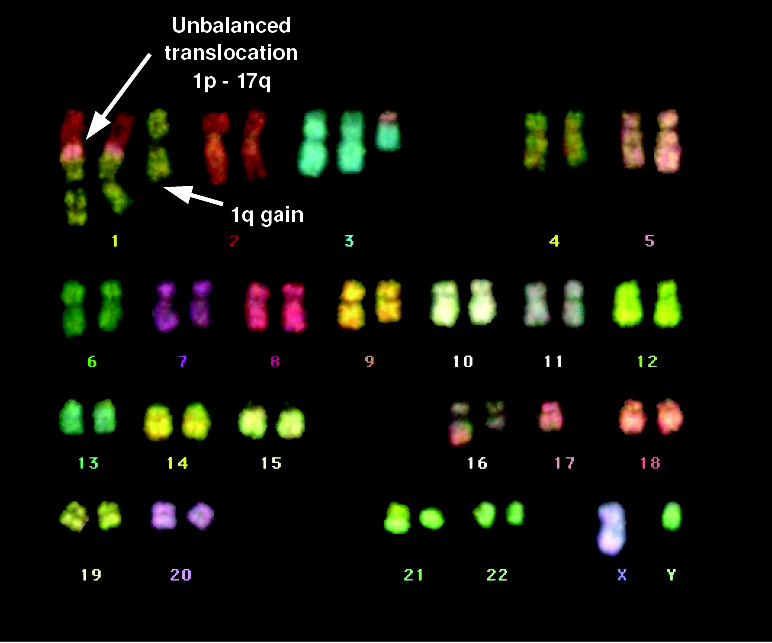
\includegraphics[height=.43\textheight]{../FIGURES/Hup08-Fig128b}
    \end{tabular}
    &
    \begin{tabular}{l}
    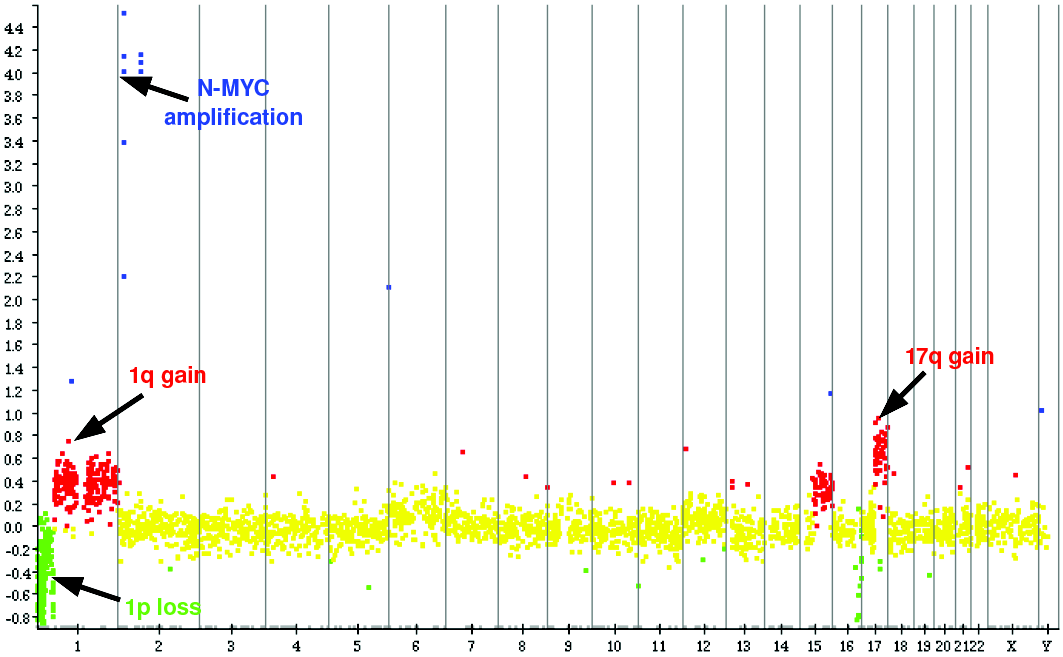
\includegraphics[height=.43\textheight]{../FIGURES/Hup08-Fig128a}
    \end{tabular}
  \end{tabular}
  $$
  \refer{Hup08}. 

}

%====================================================================
\frame{\frametitle{Recurrent alterations}

  \vspace{-.05\textheight}
  $$
  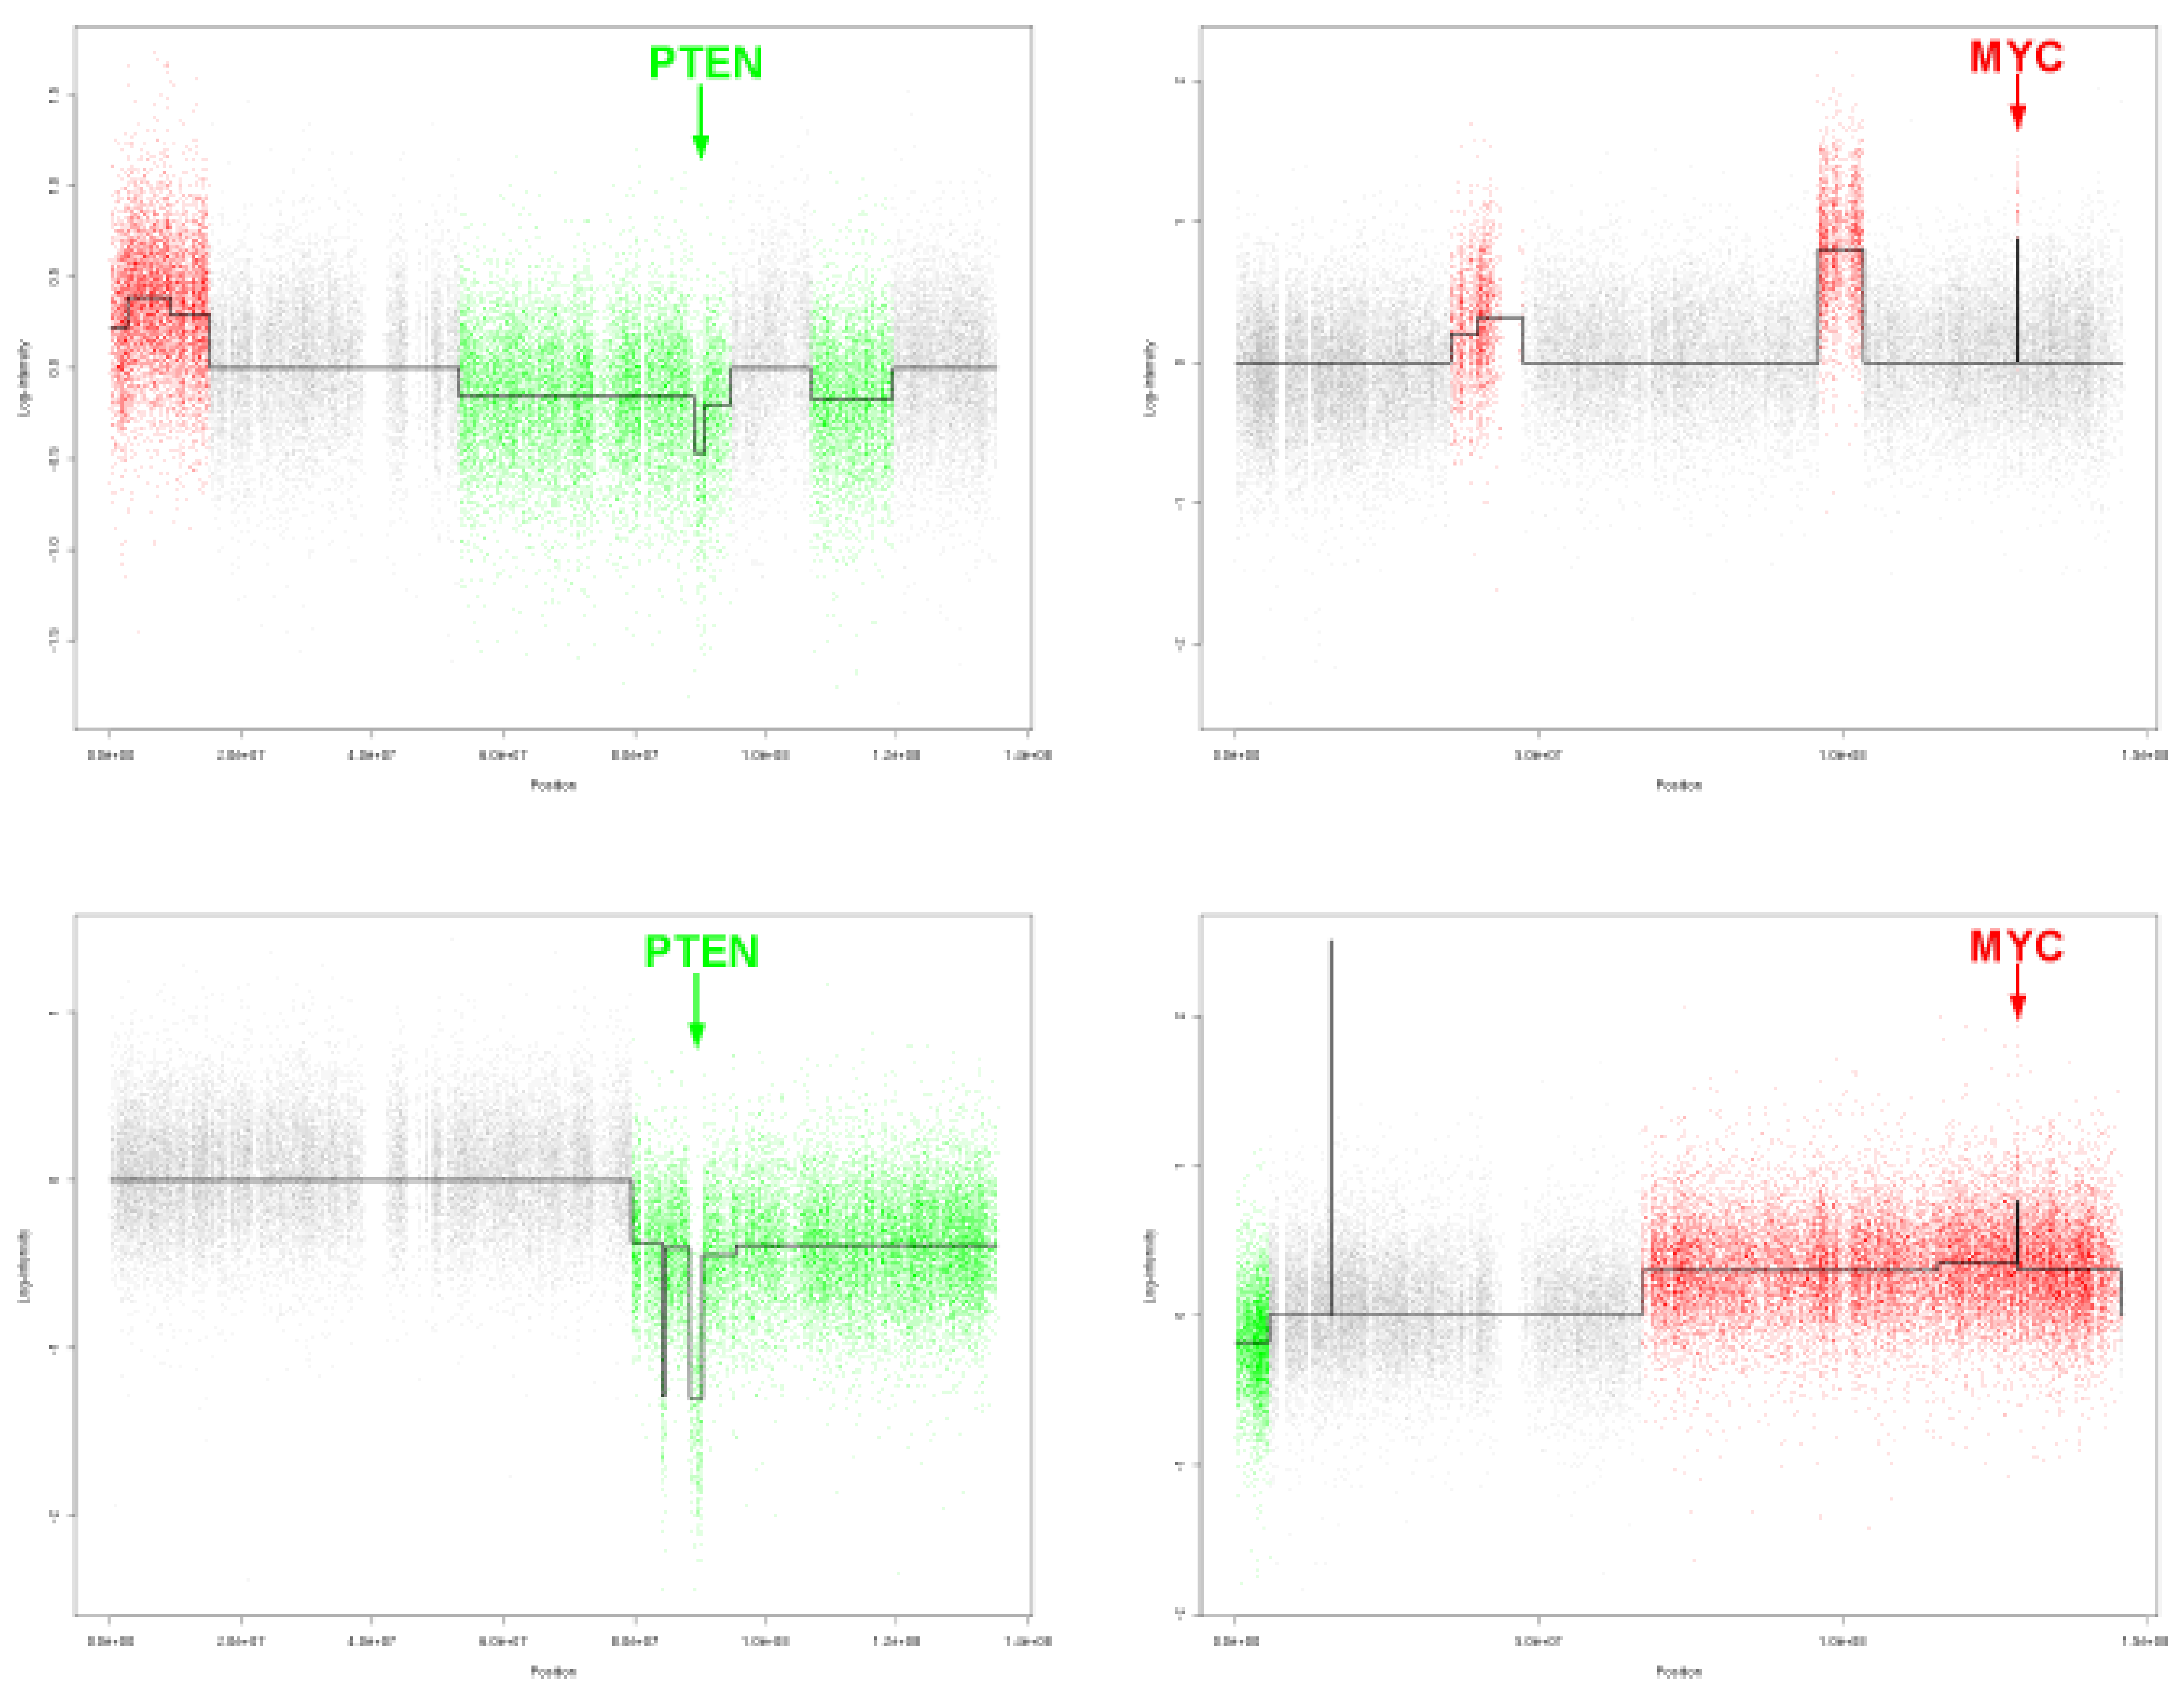
\includegraphics[height=.8\textheight]{../FIGURES/Rig10-Fig6-5}
  $$
  Chrom. 10 and 8 of two patients with breast carcinomas. \refer{Rig11} 
}


%====================================================================
%====================================================================
\section{Local scale}
%====================================================================
\frame{\frametitle{Local scale: Posterior distributions of change points} 

\begin{tabular}{cc}
    \hspace{-.5cm}
    \begin{tabular}{p{.5\textwidth}}
      {\paragraph{Bayesian framework.} 
        \begin{itemize}
        \item {$K $ number of change-points\\~}
        \item {$(\tau_k) = $ change location\\~}
        \item {$(\theta_r) = $ mean signal in region $r$\\~}
        \item {$(Y_t) =$ observed signal}
        \end{itemize}}
    \end{tabular}
    & 
    \hspace{-1cm}
    \begin{tabular}{c}
%       \onslide+<2->{
%         \hspace{-6cm}
%         \onslide+<3->{if $t \in \textcolor{blue}{r_k}$,} \quad $Y_t$
%         \onslide+<5->{$\sim
%           \Fcal($}\onslide+<4->{$\textcolor{red}{\theta_k}$}\onslide+<5->{$)$}
%         \\}
%       \begin{overprint}
%         \onslide<2>
%         \includegraphics[width=.5\textwidth]{../FIGURES/FigSeg-Budapest-1} 
%         \onslide<3>
%         \includegraphics[width=.5\textwidth]{../FIGURES/FigSeg-Budapest-2} 
%         \onslide<4>
%         \includegraphics[width=.5\textwidth]{../FIGURES/FigSeg-Budapest-3} 
%         \onslide<5>
         \includegraphics[width=.5\textwidth]{../FIGURES/FigSeg-Budapest-4} 
%         \onslide<6->
%         \includegraphics[width=.5\textwidth]{../FIGURES/FigSeg-Budapest-0} 
%       \end{overprint}
    \end{tabular}
  \end{tabular}

  {
  \paragraph{A quadratic algorithm} can be designed to compute $p(m | Y, K)$ \refer{RLR11}
  } 
  }

%====================================================================
\frame{\frametitle{Comparing transcript boundaries in yeast}

  \vspace{-.05\textheight}
  \begin{tabular}{p{.2\textwidth}p{.7\textwidth}}
    \begin{tabular}{p{.3\textwidth}}
	 One gene \\
	 \\
	 $\times$ \\
	 \\
	 Three growth \\
	 conditions: 
	 $A$, $B$, $C$
    \end{tabular}
    &
    \begin{tabular}{p{.7\textwidth}}
    \includegraphics[width=.7\textwidth]{../FIGURES/compyeastresult.pdf}
    \end{tabular}
  \end{tabular}
}

%====================================================================
\frame{\frametitle{Comparison of locations}

  3 comparisons ($A/B$, $A/C$, $B/C$) $\times$ 4 change points:
  
\centerline{\includegraphics[width=.8\textwidth, height=.8\textheight]{../FIGURES/cred-yeast.pdf}}

}

%====================================================================
\frame{\frametitle{Various isoforms in yeast?} 

  \paragraph{$P(E_0|\Ybf, \Kbf)$} for yeast genes with 2 expressed exons
  $$
  \begin{tabular}{cc}
  \includegraphics[width=.4\textwidth]{../FIGURES/statall-all} 
  & 
  \includegraphics[width=.4\textwidth]{../FIGURES/statall2} 
  \\
   $p_0 = (.5, \;.5, \;.5, \;.5)$
   &
   $p_0 = (.9, \;.99, \;.99, \;.9)$
  \end{tabular}
  $$
}

%====================================================================
%====================================================================
\section{3D conformation}
%====================================================================
\frame{\frametitle{Chromosome conformation capture}
    \begin{tabular}{p{.4\textwidth}p{.5\textwidth}}
    \begin{tabular}{p{.4\textwidth}}
	 \paragraph{Human chromosome 21} \\ ~\\
	 
	\paragraph{NGS =} nucleotide resolution \\ 
    \ra window-width $w \approx 10^5$ \\
    \ra signal: $n \approx 10^3$ \\ ~\\
  
	 Domains found by \refer{DSY12}: \\
	 HMM on directionality index \\
	 \ra good concordance with external data
    \end{tabular}
    &
    \begin{tabular}{p{.5\textwidth}}
	 %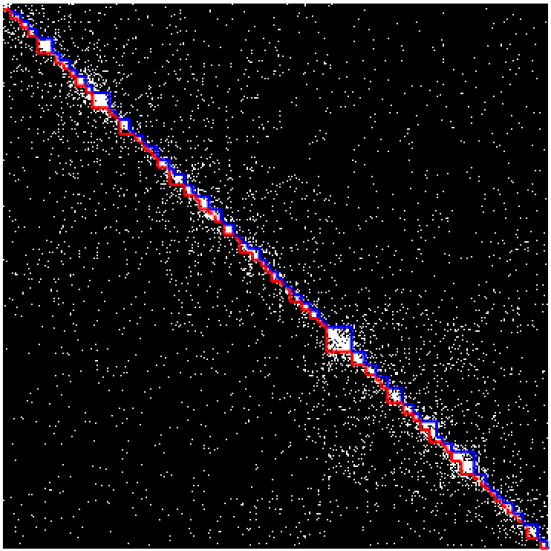
\includegraphics[height=.6\textheight]{\fignet/DLM14-JDS-Fig3}
    	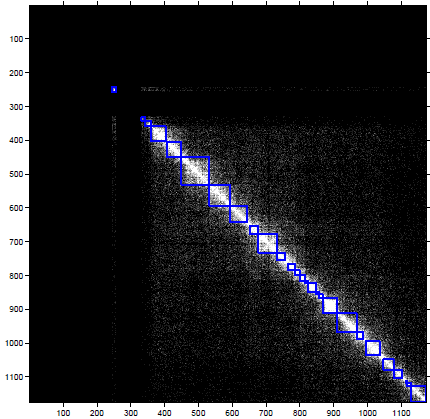
\includegraphics[width=.5\textwidth]{\fignet/DLM14-ECCB-Fig2a}
    \end{tabular}
  \end{tabular} \\~
  
  \ra A block-diagonal segmentation problem that can solved efficiently \refer{LDM14}
  }

%====================================================================
%====================================================================
\section*{References}
%====================================================================

{\tiny
  \bibliography{/home/robin/Biblio/BibGene}
  %\bibliographystyle{/home/robin/LATEX/astats}
  \bibliographystyle{plain}
  }

%====================================================================
%====================================================================
\end{document}
%====================================================================
%====================================================================


\frame{\frametitle{}
  }

